
\documentclass[journal,12pt,twocolumn]{IEEEtran}
%
\usepackage{setspace}
\usepackage{circuitikz}
\usepackage{gensymb}
\usepackage{xcolor}
\usepackage{caption}
%\usepackage{subcaption}
%\doublespacing
\singlespacing

%\usepackage{graphicx}
%\usepackage{amssymb}
%\usepackage{relsize}
\usepackage[cmex10]{amsmath}
\usepackage{mathtools}
%\usepackage{amsthm}
%\interdisplaylinepenalty=2500
%\savesymbol{iint}
%\usepackage{txfonts}
%\restoresymbol{TXF}{iint}
%\usepackage{wasysym}
\usepackage{hyperref}
\usepackage{amsthm}
\usepackage{mathrsfs}
\usepackage{txfonts}
\usepackage{stfloats}
\usepackage{cite}
\usepackage{cases}
\usepackage{subfig}
%\usepackage{xtab}
\usepackage{longtable}
\usepackage{multirow}
%\usepackage{algorithm}
%\usepackage{algpseudocode}
%\usepackage{enumerate}
\usepackage{enumitem}
\usepackage{mathtools}
%\usepackage{iithtlc}
%\usepackage[framemethod=tikz]{mdframed}
\usepackage{listings}
\let\vec\mathbf


%\usepackage{stmaryrd}


%\usepackage{wasysym}
%\newcounter{MYtempeqncnt}
\DeclareMathOperator*{\Res}{Res}
%\renewcommand{\baselinestretch}{2}
\renewcommand\thesection{\arabic{section}}
\renewcommand\thesubsection{\thesection.\arabic{subsection}}
\renewcommand\thesubsubsection{\thesubsection.\arabic{subsubsection}}

\renewcommand\thesectiondis{\arabic{section}}
\renewcommand\thesubsectiondis{\thesectiondis.\arabic{subsection}}
\renewcommand\thesubsubsectiondis{\thesubsectiondis.\arabic{subsubsection}}

%\renewcommand{\labelenumi}{\textbf{\theenumi}}
%\renewcommand{\theenumi}{P.\arabic{enumi}}

% correct bad hyphenation here
\hyphenation{op-tical net-works semi-conduc-tor}

\lstset{
language=Python,
frame=single, 
breaklines=true,
columns=fullflexible
}



\begin{document}
%

\theoremstyle{definition}
\newtheorem{theorem}{Theorem}[section]
\newtheorem{problem}{Problem}
\newtheorem{proposition}{Proposition}[section]
\newtheorem{lemma}{Lemma}[section]
\newtheorem{corollary}[theorem]{Corollary}
\newtheorem{example}{Example}[section]
\newtheorem{definition}{Definition}[section]
%\newtheorem{algorithm}{Algorithm}[section]
%\newtheorem{cor}{Corollary}
\newcommand{\BEQA}{\begin{eqnarray}}
\newcommand{\EEQA}{\end{eqnarray}}
\newcommand{\define}{\stackrel{\triangle}{=}}
\newcommand{\myvec}[1]{\ensuremath{\begin{pmatrix}#1\end{pmatrix}}}
\newcommand{\mydet}[1]{\ensuremath{\begin{vmatrix}#1\end{vmatrix}}}

\bibliographystyle{IEEEtran}
%\bibliographystyle{ieeetr}

\providecommand{\nCr}[2]{\,^{#1}C_{#2}} % nCr
\providecommand{\nPr}[2]{\,^{#1}P_{#2}} % nPr
\providecommand{\mbf}{\mathbf}
\providecommand{\pr}[1]{\ensuremath{\Pr\left(#1\right)}}
\providecommand{\qfunc}[1]{\ensuremath{Q\left(#1\right)}}
\providecommand{\sbrak}[1]{\ensuremath{{}\left[#1\right]}}
\providecommand{\lsbrak}[1]{\ensuremath{{}\left[#1\right.}}
\providecommand{\rsbrak}[1]{\ensuremath{{}\left.#1\right]}}
\providecommand{\brak}[1]{\ensuremath{\left(#1\right)}}
\providecommand{\lbrak}[1]{\ensuremath{\left(#1\right.}}
\providecommand{\rbrak}[1]{\ensuremath{\left.#1\right)}}
\providecommand{\cbrak}[1]{\ensuremath{\left\{#1\right\}}}
\providecommand{\lcbrak}[1]{\ensuremath{\left\{#1\right.}}
\providecommand{\rcbrak}[1]{\ensuremath{\left.#1\right\}}}
\providecommand{\der}[1]{\mathrm{d} #1}
\theoremstyle{remark}
\newtheorem{rem}{Remark}
\newcommand{\sgn}{\mathop{\mathrm{sgn}}}
\providecommand{\abs}[1]{\left\vert#1\right\vert}
\providecommand{\res}[1]{\Res\displaylimits_{#1}} 
\providecommand{\norm}[1]{\lVert#1\rVert}
\providecommand{\mtx}[1]{\mathbf{#1}}
\providecommand{\mean}[1]{E\left[ #1 \right]}
\providecommand{\fourier}{\overset{\mathcal{F}}{ \rightleftharpoons}}
\providecommand{\z}[1]{{\mathcal{Z}}\cbrak{#1}}
\providecommand{\ztrans}{\overset{\mathcal{Z}}{ \rightleftharpoons}}

%\providecommand{\hilbert}{\overset{\mathcal{H}}{ \rightleftharpoons}}
\providecommand{\system}{\overset{\mathcal{H}}{ \longleftrightarrow}}
	%\newcommand{\solution}[2]{\textbf{Solution:}{#1}}
\newcommand{\solution}{\noindent \textbf{Solution: }}
\providecommand{\dec}[2]{\ensuremath{\overset{#1}{\underset{#2}{\gtrless}}}}
\numberwithin{equation}{section}
%\numberwithin{equation}{subsection}
%\numberwithin{problem}{subsection}
%\numberwithin{definition}{subsection}
\makeatletter
\@addtoreset{figure}{problem}
\makeatother

\let\StandardTheFigure\thefigure
%\renewcommand{\thefigure}{\theproblem.\arabic{figure}}
\renewcommand{\thefigure}{\theproblem}


%\numberwithin{figure}{subsection}

\def\putbox#1#2#3{\makebox[0in][l]{\makebox[#1][l]{}\raisebox{\baselineskip}[0in][0in]{\raisebox{#2}[0in][0in]{#3}}}}
     \def\rightbox#1{\makebox[0in][r]{#1}}
     \def\centbox#1{\makebox[0in]{#1}}
     \def\rightarrowpbox#1{\raisebox{-\baselineskip}[0in][0in]{#1}}
     \def\midbox#1{\raisebox{-0.5\baselineskip}[0in][0in]{#1}}

\vspace{3cm}

\title{ 
%\logo{
%}
Circuits and Transforms
%	\logo{Octave for Math Computing }
}
%\title{
%	\logo{Matrix Analysis through Octave}{\begin{center}\includegraphics[scale=.24]{tlc}\end{center}}{}{HAMDSP}
%}


% paper title
% can use linebreaks \\ within to get better formatting as desired
%\title{Matrix Analysis through Octave}
%
%
% author names and IEEE memberships
% note positions of commas and nonbreaking spaces ( ~ ) LaTeX will not break
% a structure at a ~ so this keeps an author's name from being broken across
% two lines.
% use \thanks{} to gain access to the first footnote area
% a separate \thanks must be used for each paragraph as LaTeX2e's \thanks
% was not built to handle multiple paragraphs
%

\author{Jarpula Bhanu Prasad - AI21BTECH11015} %<-this  stops a space
% \thanks{*The author is with the Department
% of Electrical Engineering, Indian Institute of Technology, Hyderabad
% 502285 India e-mail:  gadepall@iith.ac.in.  All content in the manuscript is 
% released under GNU GPL.  Free to use for anything. }% <-this % stops a space
% %\thanks{J. Doe and J. Doe are with Anonymous University.}% <-this % stops a space
% %\thanks{Manuscript received April 19, 2005; revised January 11, 2007.}}
% }
% note the % following the last \IEEEmembership and also \thanks - 
% these prevent an unwanted space from occurring between the last author name
% and the end of the author line. i.e., if you had this:
% 
% \author{....lastname \thanks{...} \thanks{...} }
%                     ^------------^------------^----Do not want these spaces!
%
% a space would be appended to the last name and could cause every name on that
% line to be shifted left slightly. This is one of those "LaTeX things". For
% instance, "\textbf{A} \textbf{B}" will typeset as "A B" not "AB". To get
% "AB" then you have to do: "\textbf{A}\textbf{B}"
% \thanks is no different in this regard, so shield the last } of each \thanks
% that ends a line with a % and do not let a space in before the next \thanks.
% Spaces after \IEEEmembership other than the last one are OK (and needed) as
% you are supposed to have spaces between the names. For what it is worth,
% this is a minor point as most people would not even notice if the said evil
% space somehow managed to creep in.



% The paper headers
%\markboth{Journal of \LaTeX\ Class Files,~Vol.~6, No.~1, January~2007}%
%{Shell \MakeLowercase{\textit{et al.}}: Bare Demo of IEEEtran.cls for Journals}
% The only time the second header will appear is for the odd numbered pages
% after the title page when using the twoside option.
% 
% *** Note that you probably will NOT want to include the author's ***
% *** name in the headers of peer review papers.                   ***
% You can use \ifCLASSOPTIONpeerreview for conditional compilation here if
% you desire.




% If you want to put a publisher's ID mark on the page you can do it like
% this:
%\IEEEpubid{0000--0000/00\$00.00~\copyright~2007 IEEE}
% Remember, if you use this you must call \IEEEpubidadjcol in the second
% column for its text to clear the IEEEpubid mark.



% make the title area
\maketitle

%\newpage

\tableofcontents

%\renewcommand{\thefigure}{\thesection.\theenumi}
%\renewcommand{\thetable}{\thesection.\theenumi}

\renewcommand{\thefigure}{\theenumi}
\renewcommand{\thetable}{\theenumi}

%\renewcommand{\theequation}{\thesection}


\bigskip

\begin{abstract}
This manual provides a simple introduction to Transforms
\end{abstract}


%% Copyright (C) 2020 Saurabh Joshi
%% 
%\let\negmedspace\undefined
%\let\negthickspace\undefined

%\documentclass[journal,12pt,onecolumn]{IEEEtran}
%%\documentclass[journal,12pt,twocolumn]{IEEEtran}
%%
%\usepackage{setspace}
%\usepackage{gensymb}
%%\doublespacing
%\singlespacing
%
%%\usepackage{graphicx}
%%\usepackage{amssymb}
%%\usepackage{relsize}
%\usepackage[cmex10]{amsmath}
%%\usepackage{amsthm}
%%\interdisplaylinepenalty=2500
%%\savesymbol{iint}
%%\usepackage{txfonts}
%%\restoresymbol{TXF}{iint}
%%\usepackage{wasysym}
%\usepackage{amsthm}
%\usepackage{mathrsfs}
%\usepackage{txfonts}
%\usepackage{stfloats}
%\usepackage{cite}
%\usepackage{cases}
%\usepackage{subfig}
%%\usepackage{xtab}
%\usepackage{longtable}
%\usepackage{multirow}
%%\usepackage{algorithm}
%%\usepackage{algpseudocode}
%\usepackage{enumitem}
%\usepackage{mathtools}
%\usepackage{tikz}
%\usetikzlibrary{shapes,arrows,positioning}
%\usepackage{circuitikz}
%\usepackage{verbatim}
%\usepackage{hyperref}
%%\usepackage{stmaryrd}
%\usepackage{tkz-euclide} % loads  TikZ and tkz-base
%%\usetkzobj{all}
%\usepackage{listings}
%    \usepackage{color}                                            %%
%    \usepackage{array}                                            %%
%    \usepackage{longtable}                                        %%
%    \usepackage{calc}                                             %%
%    \usepackage{multirow}                                         %%
%    \usepackage{hhline}                                           %%
%    \usepackage{ifthen}                                           %%
%  %optionally (for landscape tables embedded in another document): %%
%    \usepackage{lscape}     
%\usepackage{multicol}
%\usepackage{chngcntr}
%\usepackage{iftex}
%%\usepackage[latin9]{inputenc}
%\usepackage{geometry}
%%\geometry{verbose,tmargin=2cm,bmargin=3cm,lmargin=1.8cm,rmargin=1.5cm,headheight=2cm,headsep=2cm,footskip=3cm}
%\usepackage{array}
%\newcolumntype{L}[1]{>{\raggedright\let\newline\\\arraybackslash\hspace{0pt}}m{#1}}
%\newcolumntype{C}[1]{>{\centering\let\newline\\\arraybackslash\hspace{0pt}}m{#1}}
%\newcolumntype{R}[1]{>{\raggedleft\let\newline\\\arraybackslash\hspace{0pt}}m{#1}}
% \usepackage{float}
%%\usepackage{graphicx}
%%\usepackage{setspace}
%%\usepackage{parskip}
%
%\def \hsp {\hspace{3mm}}
%
%\makeatletter
%
%\providecommand{\tabularnewline}{\\}
%
%
%\makeatother
%\ifxetex
%\usepackage[T1]{fontenc}
%\usepackage{fontspec}
%%\setmainfont[ Path = fonts/]{Sanskrit_2003.ttf}
%\newfontfamily\nakulafont[Script=Devanagari,AutoFakeBold=2,Path = fonts/]{Nakula}
%%\newfontfamily\liberationfont{Liberation Sans Narrow}
%%\newfontfamily\liberationsansfont{Liberation Sans}
%\fi
%\usepackage{tikz}
%\usepackage{xcolor}
%%\usepackage{enumerate}
%
%%\usepackage{wasysym}
%%\newcounter{MYtempeqncnt}
%\DeclareMathOperator*{\Res}{Res}
%%\renewcommand{\baselinestretch}{2}
%\renewcommand\thesection{\arabic{section}}
%\renewcommand\thesubsection{\thesection.\arabic{subsection}}
%\renewcommand\thesubsubsection{\thesubsection.\arabic{subsubsection}}
%
%\renewcommand\thesectiondis{\arabic{section}}
%\renewcommand\thesubsectiondis{\thesectiondis.\arabic{subsection}}
%\renewcommand\thesubsubsectiondis{\thesubsectiondis.\arabic{subsubsection}}
%
%% correct bad hyphenation here
%\hyphenation{op-tical net-works semi-conduc-tor}
%\def\inputGnumericTable{}                                 %%
%
%\lstset{
%language=tex,
%frame=single, 
%breaklines=true
%}
%
%%\begin{document}
%%
%
%
%\newtheorem{theorem}{Theorem}[section]
%\newtheorem{problem}{Problem}
%\newtheorem{proposition}{Proposition}[section]
%\newtheorem{lemma}{Lemma}[section]
%\newtheorem{corollary}[theorem]{Corollary}
%\newtheorem{example}{Example}[section]
%\newtheorem{definition}[problem]{Definition}
%%\newtheorem{thm}{Theorem}[section] 
%%\newtheorem{defn}[thm]{Definition}
%%\newtheorem{algorithm}{Algorithm}[section]
%%\newtheorem{cor}{Corollary}
%\newcommand{\BEQA}{\begin{eqnarray}}
%\newcommand{\EEQA}{\end{eqnarray}}
%\newcommand{\define}{\stackrel{\triangle}{=}}
%
%\bibliographystyle{IEEEtran}
%%\bibliographystyle{ieeetr}
%
%
%\providecommand{\mbf}{\mathbf}
%\providecommand{\pr}[1]{\ensuremath{\Pr\left(#1\right)}}
%\providecommand{\qfunc}[1]{\ensuremath{Q\left(#1\right)}}
%\providecommand{\sbrak}[1]{\ensuremath{{}\left[#1\right]}}
%\providecommand{\lsbrak}[1]{\ensuremath{{}\left[#1\right.}}
%\providecommand{\rsbrak}[1]{\ensuremath{{}\left.#1\right]}}
%\providecommand{\brak}[1]{\ensuremath{\left(#1\right)}}
%\providecommand{\lbrak}[1]{\ensuremath{\left(#1\right.}}
%\providecommand{\rbrak}[1]{\ensuremath{\left.#1\right)}}
%\providecommand{\cbrak}[1]{\ensuremath{\left\{#1\right\}}}
%\providecommand{\lcbrak}[1]{\ensuremath{\left\{#1\right.}}
%\providecommand{\rcbrak}[1]{\ensuremath{\left.#1\right\}}}
%\theoremstyle{remark}
%\newtheorem{rem}{Remark}
%\newcommand{\sgn}{\mathop{\mathrm{sgn}}}
%\providecommand{\abs}[1]{\left\vert#1\right\vert}
%\providecommand{\res}[1]{\Res\displaylimits_{#1}} 
%\providecommand{\norm}[1]{\left\lVert#1\right\rVert}
%%\providecommand{\norm}[1]{\lVert#1\rVert}
%\providecommand{\mtx}[1]{\mathbf{#1}}
%\providecommand{\mean}[1]{E\left[ #1 \right]}
%\providecommand{\fourier}{\overset{\mathcal{F}}{ \rightleftharpoons}}
%%\providecommand{\hilbert}{\overset{\mathcal{H}}{ \rightleftharpoons}}
%%\providecommand{\system}{\overset{\mathcal{H}}{ \longleftrightarrow}}
%\providecommand{\system}[1]{\overset{\mathcal{#1}}{ \longleftrightarrow}}
%\newcommand{\sinc}{\,\text{sinc}\,}
%\newcommand{\rect}{\,\text{rect}\,}
%	%\newcommand{\solution}[2]{\textbf{Solution:}{#1}}
%\newcommand{\solution}{\noindent \textbf{Solution: }}
%\newcommand{\cosec}{\,\text{cosec}\,}
%\providecommand{\dec}[2]{\ensuremath{\overset{#1}{\underset{#2}{\gtrless}}}}
%\newcommand{\myvec}[1]{\ensuremath{\begin{pmatrix}#1\end{pmatrix}}}
%\newcommand{\mydet}[1]{\ensuremath{\begin{vmatrix}#1\end{vmatrix}}}
%\newcommand*{\permcomb}[4][0mu]{{{}^{#3}\mkern#1#2_{#4}}}
%\newcommand*{\perm}[1][-3mu]{\permcomb[#1]{P}}
%\newcommand*{\comb}[1][-1mu]{\permcomb[#1]{C}}
%%\numberwithin{equation}{section}
%\numberwithin{equation}{section}
%%\numberwithin{problem}{section}
%%\numberwithin{definition}{section}
%\makeatletter
%\@addtoreset{figure}{problem}
%\makeatother
%
%\let\StandardTheFigure\thefigure
%\let\vec\mathbf
%%\renewcommand{\thefigure}{\theproblem.\arabic{figure}}
%\renewcommand{\thefigure}{\theproblem}
%%\setlist[enumerate,1]{before=\renewcommand\theequation{\theenumi.\arabic{equation}}
%%\counterwithin{equation}{enumi}
%
%
%%\renewcommand{\theequation}{\arabic{subsection}.\arabic{equation}}
%
%\vspace{3cm}
%
%
%%\usepackage{babel}
%\begin{document}
%
%\begin{tabular}{L{6cm} C{2cm} R{5cm} }
%
%	\definecolor{circleorange}{rgb}{1,0.17,0.08}
%\definecolor{darkorange}{rgb}{1,0.27,0.1}
%\definecolor{orange2}{rgb}{1,0.5,0.15}
%\definecolor{orange3}{rgb}{1,0.65,0.25}
%\definecolor{yellow1}{rgb}{0.95,0.77,0.2}
%%\begin{tikzpicture}[scale=0.2,every node/.style={transform shape}]
%\begin{tikzpicture}[scale=0.1,every node/.style={transform shape}]
%\draw [fill=circleorange,circleorange] (5,10) circle (1.15); 
%\fill [darkorange] (5.06,8) -- (5.06,2) -- (7.3,1.2) -- (7.3,8.8) -- (5.06,8);
%\fill [darkorange] (4.94,8) -- (4.94,2) -- (2.7,1.2) -- (2.7,8.8) -- (4.94,8);
%\fill [orange2]    (7.4,8.4) -- (7.4,1.6) -- (8.2,1.2) -- (8.2,8.8) -- (7.4,8.4);
%\fill [orange2]    (2.6,8.4) -- (2.6,1.6) -- (1.8,1.2) -- (1.8,8.8) -- (2.6,8.4);
%\fill [orange3]    (8.3,8.4) -- (8.3,1.6) -- (9.0,1.2) -- (9.0,8.8) -- (8.3,8.4);
%\fill [orange3]    (1.7,8.4) -- (1.7,1.6) -- (1.0,1.2) -- (1.0,8.8) -- (1.7,8.4);
%\fill [yellow1]    (9.1,8.4) -- (9.1,1.6) -- (9.7,1.2) -- (9.7,8.8) -- (9.1,8.4);
%\fill [yellow1]    (0.9,8.4) -- (0.9,1.6) -- (0.3,1.2) -- (0.3,8.8) -- (0.9,8.4);
%\ifxetex
%\node [scale=2.1] at (5,-0.1)  {   {\bf {\nakulafont  भारतीय प्रौद्योगिकी संस्थान हैदराबाद }} };
%\node [scale=1.8] at (5,-1.2) {   {\bf { Indian Institute of Technology Hyderabad}} };
%%\node [scale=1.8] at (5,-1.2) {   {\bf {\liberationsansfont Indian Institute of Technology Hyderabad}} };
%\fi
%\end{tikzpicture}
%% \includegraphics[scale=0.05]{logo_iith} \newline
%
%& Quiz  13
%	&
%EE3900	
%\end{tabular}
%
%
%\vspace{-6mm}
%\begin{center}
%%\includegraphics[scale=0.95]{Yellow-Line}
%\begin{tikzpicture}
%\definecolor{yellow1}{rgb}{0.95,0.77,0.2}
%\draw[line width=0.75mm, yellow1] (0,0) -- (\textwidth,0);
%\end{tikzpicture}
%\par\end{center}

 \section{Definitions}
\begin{enumerate}[label=\arabic*.,ref=\thesection.\theenumi]
\numberwithin{equation}{section}
\numberwithin{figure}{section}
\item The unit step function is 
\begin{align}
u(t) =
\begin{cases}
1 & t > 0
\\
	\frac{1}{2} & t = 0
\\
0 & t < 0
\end{cases}
\end{align}
\item The Laplace transform of $g(t)$ is defined as 
\begin{align}
	G(s) = \int_{-\infty}^{\infty} g(t) e^{-st}\, dt
\end{align}
 \end{enumerate}

 \section{Laplace Transform}
\begin{enumerate}[label=\arabic*.,ref=\thesection.\theenumi]
\numberwithin{equation}{section}
\item In the circuit, the switch S is connected to position P for a long time so that the charge on the capacitor
	becomes $q_1 \, \mu C$. Then S is switched to position Q.  After a long time, the charge on the capacitor is
		$q_2 \, \mu C$.
		\begin{figure}[!ht]
			\centering
			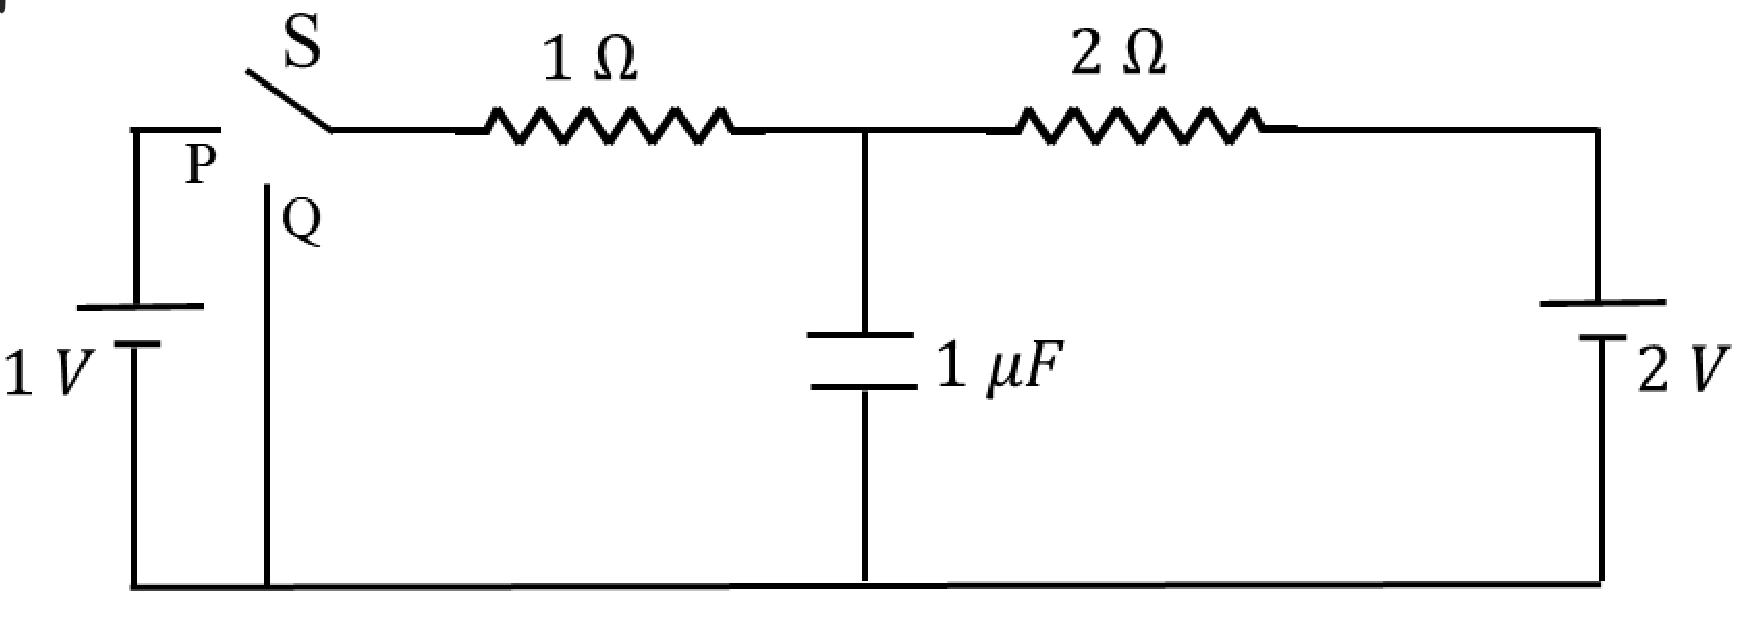
\includegraphics[width=\columnwidth]{figs/ckt.jpg}
			\caption{}
			\label{fig:ckt}
\end{figure}
\item Draw the circuit using latex-tikz.\\
\solution The circuit drawn using the latex-tikz is Fig.\eqref{fig:ckt-q2} \\
When switch is closed at position P
\begin{figure}[!ht]
    \begin{circuitikz} \draw
        (0,0) to[battery1, l=1 $V$, invert] (0,2)
        -- (0.8,2) node[label={above:P}] {}
        to[R, l^=$1 \Omega$, *-*] (3,2) 
        node[label={above:A}] {}
        to[R, l^=$2 \Omega$] (5.5,2)
        to[battery1, l=2 $V$] (5.5,0)
        -- (0,0)
        (3,2) to[C, l=1 ${\mu}F$] (3,0)
        -- (0.8,0) to (0.8,1.6) node[ocirc,label=right:Q] {};
    \end{circuitikz}
    \caption{}
    \label{fig:ckt-q2}
\end{figure}
\item Find $q_1$.\\
\solution When the switch is closed for long time the circuit achives steady state condition.\\
Then the equivalent circuit is given by
\begin{figure}[!ht]
    \begin{circuitikz} \draw
        (0,0) to[battery1, l=1 $V$, invert] (0,2)
        -- (0.8,2) node[label={above:P}] {}
        to[R, l^=$1 \Omega$, *-*] (3,2) 
        node[label={above:A}] {}
        to[R, l^=$2 \Omega$] (5.5,2)
        to[battery1, l=2 $V$] (5.5,0)
        -- (0,0) {};
    \end{circuitikz}
    \caption{}
    \label{fig:ckt-q3}
\end{figure}\\
consider the circuit as cells with internal resistors connected in series.
\begin{align}
    i = \frac{V}{R_{eq}} = \frac{1}{1+2} = \frac{1}{3}A
\end{align}
Now voltage across 2$\Omega$ resistro is given by
\begin{align}
    \implies \quad 2-V_A &= \frac{1}{3}\times 2 = \frac{2}{3}\\
    V_A &= 2 - \frac{2}{3}\\
    &= \frac{4}{3} 
\end{align}

 Now, charge 
 \begin{align}
    q_1 &= C\Delta V\\
    &= 1 \times \frac{4}{3}\\
    &=\frac{4}{3}
 \end{align}
 charge on $q_1$ is $\frac{4}{3} \mu C$
	\item Show that the Laplace transform of $u(t)$ is $\frac{1}{s}$ and find the ROC.\\
	\solution \begin{align}
        \mathcal{L}[u(t)] &= U(s) =\int_{-\infty}^{\infty} u(t) e^{-st}dt\\
        U(s) &= \int_{0}^0 \frac{1}{2}e^{-st}dt + \int_0^{\infty} 1e^{-st} dt\\
        &= -\frac{1}{s}\abs{e^{-st}}_0^{\infty}\\
        &= -\frac{1}{s} \sbrak{e^{-s\infty}-e^{-s\times 0}}
    \end{align}
    The above term converges if and only if $e^{-st} \rightarrow 0$ as $ t \rightarrow \infty$ only possible if $Re\cbrak{s}>0$.\\
    hence 
    \begin{equation}
        U(s) = \frac{1}{s} \qquad Re\cbrak{s}>0
    \end{equation}
	\item Show that 
		\begin{align}
			e^{-at}u(t) \system{L} \frac{1}{s+a}, \quad a > 0
		\end{align}
		and find the ROC.\\
        \solution
        Let $x(t) = e^{-at}u(t)$
        \begin{align}
            \mathcal{L}[x(t)] &= X(s) =\int_{-\infty}^{\infty}e^{-at} u(t) e^{-st}dt\\
            &=\int_{-\infty}^{\infty}e^{-(s+a)t} u(t)dt\\
            X(s) &= \int_{0}^0 \frac{1}{2}e^{-(s+a)t}dt + \int_0^{\infty} 1 e^{-(s+a)t}dt\\
            &= -\frac{1}{s+a}\abs{e^{-(s+a)t}}_0^{\infty}\\
            &= -\frac{1}{s+a} \sbrak{e^{-(s+a)\infty}-e^{-(s+a)\times 0}}
        \end{align}
        The above term converges if and only if $e^{-(s+a)t} \rightarrow 0$ as $ t \rightarrow \infty$ only possible if $Re\cbrak{s}>-a$.\\
        hence 
        \begin{equation}
            X(s) = \frac{1}{s+a} \qquad Re\cbrak{s}>-a
        \end{equation}
	\item Now consider the following resistive circuit transformed from 
			Fig. \ref{fig:ckt}
		\begin{figure}[!ht]
			\centering
			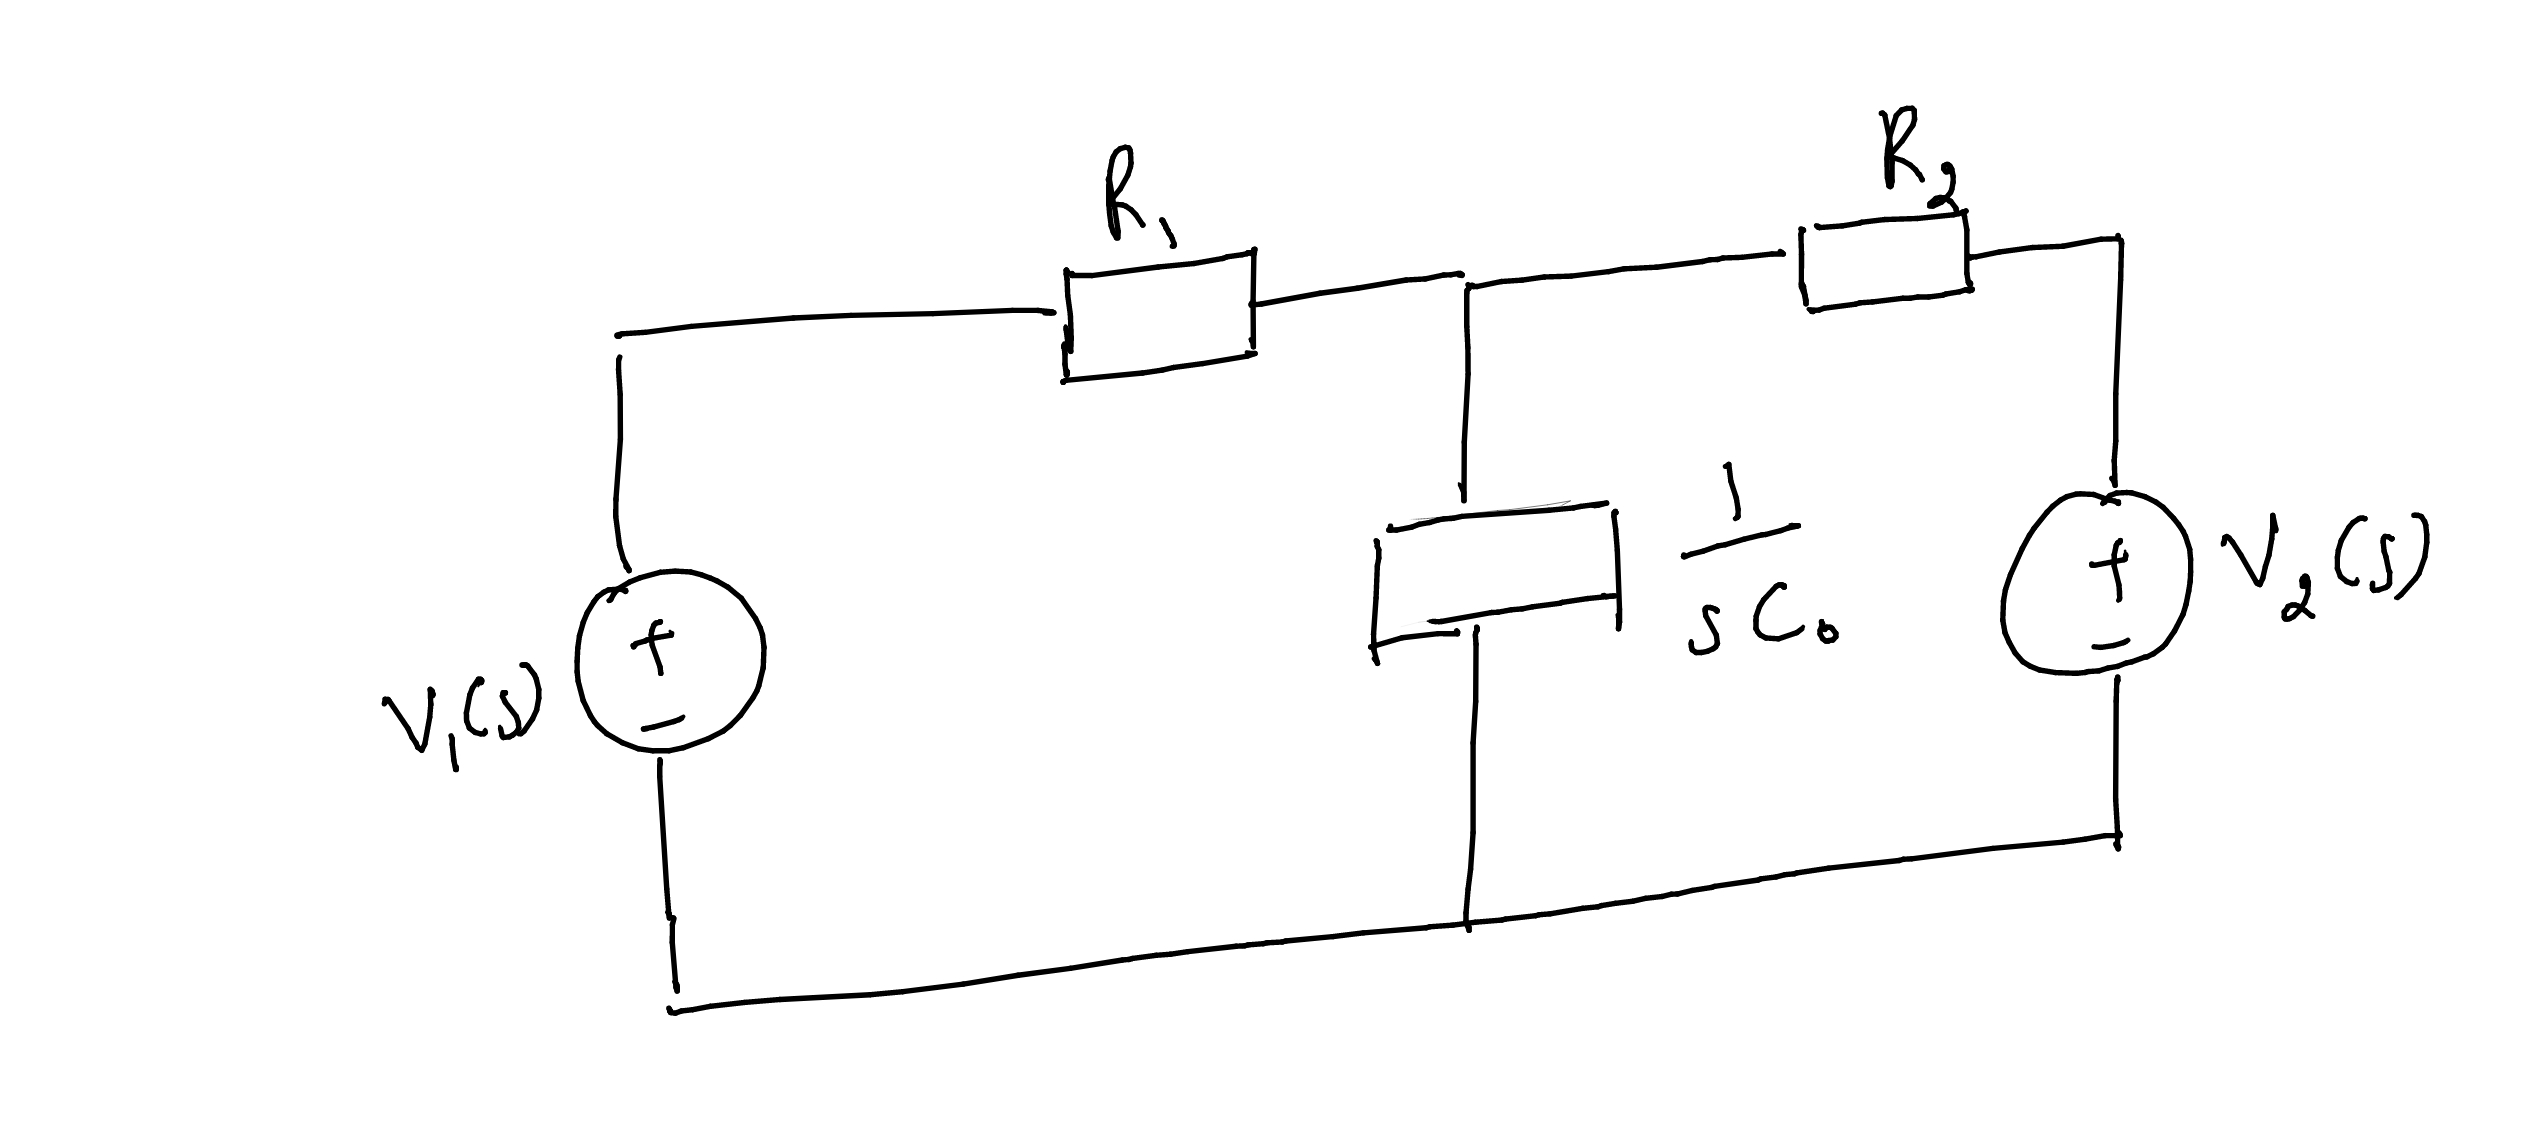
\includegraphics[width=\columnwidth]{figs/lap-ckt.jpg}
			\caption{}
			\label{fig:lap-ckt}
\end{figure}
		where 
		\begin{align}
			u(t) \system{L} V_1(s)
			\\
			2u(t) \system{L} V_2(s)
		\end{align}
		Find the voltage across the capacitor $V_{C_0}(s)$.\\
        \solution We see that
        \begin{align}
            V_1(s) = \frac{1}{s} \qquad
            V_2(s) = \frac{2}{s}
        \end{align}
        In Fig. \ref{fig:ckt-q2}, we use KCL at A.
        \begin{align}
            &\frac{V - \frac{1}{s}}{R_1} + \frac{V - \frac{2}{s}}{R_2} + sC_0V = 0 \\
            &V\brak{\frac{1}{R_1} + \frac{1}{R_2} + sC_0} = \frac{1}{s}\brak{\frac{1}{R_1} + \frac{2}{R_2}} \\
            &V(s) = \frac{\frac{1}{R_1} + \frac{2}{R_2}}{s\brak{\frac{1}{R_1} + \frac{1}{R_2} + sC_0}} \\
            &= \frac{\frac{1}{R_1} + \frac{2}{R_2}}{\frac{1}{R_1} + \frac{1}{R_2}}\brak{\frac{1}{s} - \frac{1}{\frac{1}{C_0}\brak{\frac{1}{R_1} + \frac{1}{R_2}} + s}} 
            \label{eq:V-s}
        \end{align}
	\item Find $v_{C_0}(t)$.  Plot using python.\\
	\solution Taking the inverse Laplace transform in \eqref{eq:V-s},
    \begin{align}
        &V(s) \system{L} \frac{2R_1 + R_2}{R_1 + R_2}u(t)\brak{1 - e^{-\brak{\frac{1}{R_1} + \frac{1}{R_2}}\frac{t}{C_0}}} \\
        &= \frac{4}{3}\brak{1 - e^{-\brak{1.5 \times 10^6}t}}u(t)
    \end{align}
    The following code will plot the graph Fig.\eqref{fig:v1-t}
    \begin{lstlisting}
wget https://github.com/jarpula-Bhanu/EE3900/blob/main/Cktsig/codes/2.7.py
    \end{lstlisting}
        run the above code using the command
        \begin{lstlisting}
        python3 2.7.py
        \end{lstlisting}
    \begin{figure}[!ht]
        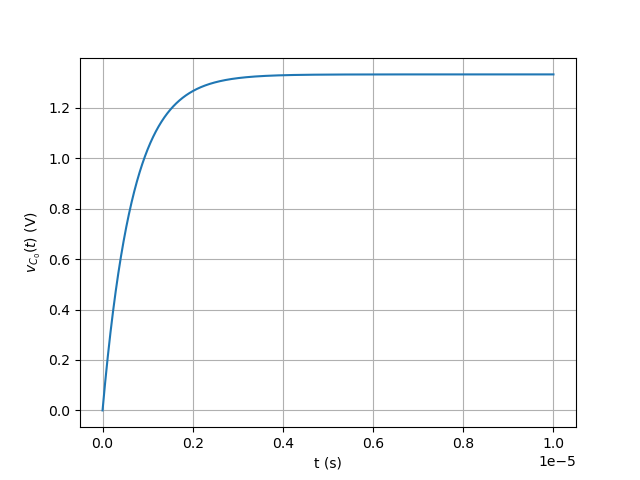
\includegraphics[width=\columnwidth]{./figs/2.7.png}
        \caption{$v_{C_0}(t)$ before the switch is flipped}
        \label{fig:v1-t}
    \end{figure}

	\item Verify your result using ngspice.\\
	\solution  The follwoing code will generate the text file of stimulation.
    \begin{lstlisting}
wget https://github.com/jarpula-Bhanu/EE3900/blob/main/Cktsig/codes/2.8.cir
    \end{lstlisting}
    The following code will plot the graph Fig.\eqref{fig:v1-ts}
    \begin{lstlisting}
wget https://github.com/jarpula-Bhanu/EE3900/blob/main/Cktsig/codes/2.8.py
    \end{lstlisting}
        run the above code using the command
        \begin{lstlisting}
        python3 2.8.py
        \end{lstlisting}
    \begin{figure}[!ht]
        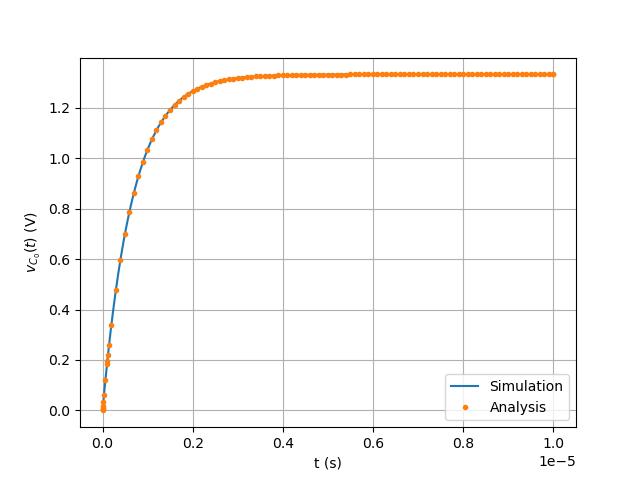
\includegraphics[width=\columnwidth]{./figs/2.8.png}
        \caption{$v_{C_0}(t)$ before the switch is flipped}
        \label{fig:v1-ts}
    \end{figure}
	\item Obtain Fig. 
			\ref{fig:lap-ckt}
			using the equivalent differential equation.
\end{enumerate}

 \section{Initial Conditions}
\begin{enumerate}[label=\arabic*.,ref=\thesection.\theenumi]
\numberwithin{equation}{section}
\item Find $q_2$ in Fig. 
			\ref{fig:ckt}.\\
\solution  When the switch is closed for long time the circuit achives steady state condition.\\
Then the equivalent circuit is given by
\begin{figure}[!ht]
    \begin{circuitikz} \draw
        -- (0,2) node[label={above:Q}] {}
        to[R, l^=$1 \Omega$, *-*] (3,2) 
        node[label={above:A}] {}
        to[R, l^=$2 \Omega$] (5.5,2)
        to[battery1, l=2 $V$] (5.5,0)
        -- (0,0)
        -- (0,0) to (0,2)  {};
    \end{circuitikz}
    \caption{}
    \label{fig:ckt-q1}
\end{figure}
Since capacitor behaves as an open circuit, we use KCL at A.
\begin{align}
    \frac{V - 0}{1} + \frac{V - 2}{2} = 0
    \implies V = \frac{2}{3}{V}
\end{align}                                         
and hence, $q_2 = \frac{2}{3}{\mu C}$.
\item Draw the equivalent $s$-domain resistive circuit when S is switched to position Q.  Use variables $R_1, R_2, C_0$ for the passive elements.
Use latex-tikz.\\
		\label{prob:init}
        \solution \begin{figure}[!htb]
            \begin{center}
            \begin{circuitikz} 
            \ctikzset{resistor = european}
            \draw
            (0,0) -- (0,3)
            node[label={above:Q}] {}
            to[R, l^=$R_1$, *-*] (3,3) 
            node[label={above:A}] {}
            to[R, l^=$R_2$] (5.5,3)
            to[battery1, l= $\frac{2}{s} V$] (5.5,0)
            -- (0,0)
            (3,3) to[battery1, l=$\frac{4}{3s} V$] (3,2) to[R, l=$\frac{1}{sC_0}$] (3,0) 
            -- (3,-0.5) node[ground, label={right:G}] {};
            \end{circuitikz}
            \end{center}
        \caption{}
        \label{fig:sckt-q2}
        \end{figure}
	
		\item $V_{C_0}(s)$ = ?  \\
        \solution Using KCL at node A in Fig. \ref{fig:sckt-q2}
\begin{align}
    \frac{V - 0}{R_1} + \frac{V - \frac{2}{s}}{R_2} + sC_0\brak{V - \frac{4}{3s}} = 0 \\
\implies V_{C_0}(s) = \frac{\frac{2}{sR_2} + \frac{4C_0}{3}}{\frac{1}{R_1} + \frac{2}{R_2} + sC_0}
\label{eq:v2-s}
\end{align}
	\item $v_{C_0}(t)$ = ? Plot using python.\\
	\solution From \eqref{eq:v2-s},
    \begin{align}
        &V_{C_0}(s) = \frac{4}{3}\brak{\frac{1}{\frac{1}{C_0}\brak{\frac{1}{R_1} + \frac{1}{R_2}}+s}} \nonumber \\
        &+ \frac{2}{R_2\brak{\frac{1}{R_1} +\frac{1}{R_2}}}\brak{\frac{1}{s} - \frac{1}{\frac{1}{C_0}\brak{\frac{1}{R_1} + \frac{1}{R_2}} + s}}
    \end{align}
    Taking an inverse Laplace Transform,
    \begin{align}
        &v_{C_0}(t) = \frac{4}{3}e^{-\brak{\frac{1}{R_1} + \frac{1}{R_2}}\frac{t}{C_0}}u(t) \nonumber \\ 
        &+ \frac{2}{R_2\brak{\frac{1}{R_1}+\frac{1}{R_2}}}\brak{1 - e^{-\brak{\frac{1}{R_1} + \frac{1}{R_2}}\frac{t}{C_0}}}u(t)
    \end{align}
    Substituting values gives
    \begin{align}
        v_{C_0}(t) = \frac{2}{3}\brak{1 +e^{-\brak{1.5 \times 10^6}t}}u(t)
        \label{eq:v2-t}
    \end{align}
    The following code will plot the graph Fig.\eqref{fig:v2-t}
    \begin{lstlisting}
wget https://github.com/jarpula-Bhanu/EE3900/blob/main/Cktsig/codes/3.4.py
    \end{lstlisting}
        run the above code using the command
        \begin{lstlisting}
        python3 3.4.py
        \end{lstlisting}
    \begin{figure}[!ht]
        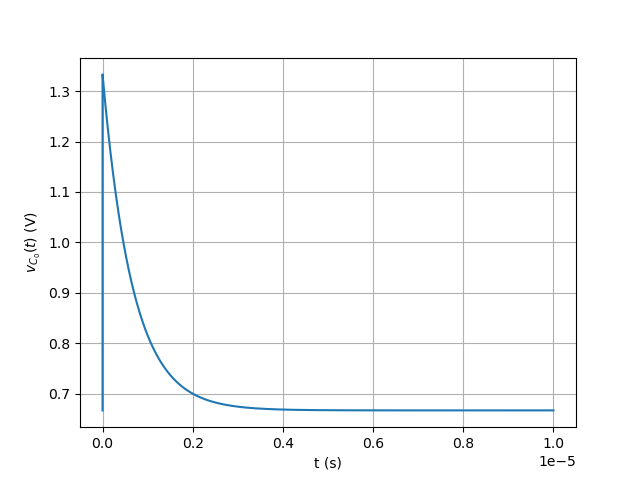
\includegraphics[width=\columnwidth]{./figs/3.4.png}
        \caption{$v_{C_0}(t)$ after the switch is flipped}
        \label{fig:v2-t}
    \end{figure}
	\item Verify your result using ngspice.\\
	\solution  The follwoing code will generate the text file of stimulation.
    \begin{lstlisting}
wget https://github.com/jarpula-Bhanu/EE3900/blob/main/Cktsig/codes/3.5.cir
    \end{lstlisting}
    The following code will plot the graph Fig.\eqref{fig:v2-ts}
    \begin{lstlisting}
wget https://github.com/jarpula-Bhanu/EE3900/blob/main/Cktsig/codes/3.5.py
    \end{lstlisting}
        run the above code using the command
        \begin{lstlisting}
        python3 3.5.py
        \end{lstlisting}
    \begin{figure}[!ht]
        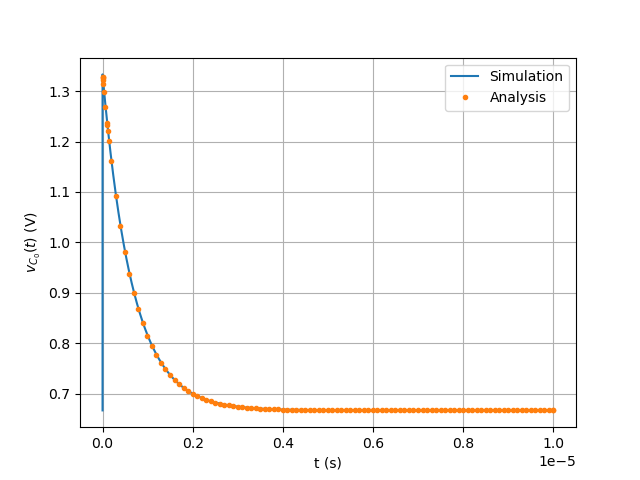
\includegraphics[width=\columnwidth]{./figs/3.5.png}
        \caption{$v_{C_0}(t)$ after the switch is flipped}
        \label{fig:v2-ts}
    \end{figure}
	\item Find $v_{C_0}(0-), v_{C_0}(0+)$ and  $v_{C_0}(\infty) $.\\
\solution From the initial conditions,
\begin{align}
    v_{C_0}(0-) &= \frac{q_1}{C} = \frac{4}{3}{V}\\
    v_{C_0}(0+) &= \lim_{t \rightarrow 0+}v_{C_0}(t) = \frac{4}{3}{V} 
\end{align}
Using \eqref{eq:v2-t},
\begin{align}
    v_{C_0}(\infty) &= \lim_{t \rightarrow \infty}v_{C_0}(t) = \frac{2}{3}{V}
\end{align}
	\item Obtain the Fig.  in problem 
		\ref{prob:init}
			using the equivalent differential equation.

            \solution Using Kirchoff's junction law
            \begin{align}
                \frac{v_c(t) - 0}{R_1} + \frac{v_c(t) - v_2(t)}{R_2} + \frac{\der{q}}{\der{t}} = 0
            \end{align}
            where $q(t)$ is the charge on the capacitor
            
            On taking the Laplace transform on both sides of this equation
            \begin{align}
                \frac{V_c(s) - 0}{R_1} + \frac{V_c(s) - V_2(s)}{R_2} + \brak{sQ(s) - q(0^-)} = 0
            \end{align}
            
            But $q(0^-) = \frac43 C_0$ and 
            \begin{align}
                q(t) &= C_0v_c(t) \\
                \implies Q(s) &= C_0V_c(s)
            \end{align}
            
            Thus
            \begin{align}
                &\frac{V_c(s) - 0}{R_1} + \frac{V_c(s) - V_2(s)}{R_2} + \brak{sC_0V_c(s) - \frac43 C_0} = 0 \\
                \implies &\frac{V_c(s) - 0}{R_1} + 	\frac{V_c(s) - V_2(s)}{R_2} + \frac{V_c(s) - \frac{4}{3s}}{\frac{1}{sC_0}} = 0 
            \end{align}
            
            which is the same equation as the one we obtained from Fig. \ref{prob:init}
            \end{enumerate}
            
            \section{Bilinear Transform}
            \begin{enumerate}[label=\thesection.\arabic*.,ref=\thesection.\theenumi]
            \item In Fig. \ref{fig:ckt}, consider the case when $S$ is switched to $Q$ right in the beginning. Formulate the differential equation
            
            \solution The equivalent circuit in the $t$-domain is shown below.
	
            \begin{figure}[!htb]
                \begin{center}
                \begin{circuitikz} 
                \draw
                (0,0) -- (0,3)
                node[label={above:Q}] {}
                to[R, l^=$R_1$, *-*, i = $i_1$] (3,3) 
                node[label={above:X}] {}
                to[R, l^=$R_2$, i = $i_3$] (5.5,3)
                to[battery1, l= $V_2$] (5.5,0)
                -- (0,0)
                (3,3) to[C, l=$C_0$, i = $i_2$] (3,0) ;
                \end{circuitikz}
                \end{center}
            \caption{}
            \label{fig:tckt-q4}
            \end{figure}
            The differential equation is the same as before 
            \begin{align}
                &\frac{v_c(t) - 0}{R_1} + \frac{v_c(t) - v_2(t)}{R_2} + \frac{\der{q}}{\der{t}} = 0 \\
                \text{i.e., } &\frac{v_c(t)}{R_1} + \frac{v_c(t) - v_2(t)}{R_2} + C_0\frac{\der{v_c}}{\der{t}} = 0
            \end{align}
            
            but with a different initial condition
            \begin{equation}
                q(0^-) = q(0) = 0
            \end{equation}
            
            \item Find $H(s)$ considering the ouput voltage at the capacitor
            
            \solution
            Transforming Fig. \ref{fig:tckt-q4} to the $s$-domain,
\begin{figure}[!htb]
    \begin{center}
    \begin{circuitikz} 
    \ctikzset{resistor = european}
    \draw
    (0,0) -- (0,3)
    node[label={above:Q}] {}
    to[R, l^=$R_1$, *-*] (3,3) 
    node[label={above:X}] {}
    to[R, l^=$R_2$] (5.5,3)
    to[battery1, l= $V_2(s)$] (5.5,0)
    -- (0,0)
    (3,3) to[R, l=$\frac{1}{sC_0}$] (3,0) 
    -- (3,-0.5) node[ground, label={right:G}] {};
    \end{circuitikz}
    \end{center}
\caption{}
\label{fig:sckt-q4}
\end{figure}
            On taking the Laplace transform on both sides of this equation
            \begin{align}
                &\frac{V_c(s)}{R_1} + \frac{V_c(s) - V_2(s)}{R_2} + sQ(s) - 0 = 0 \\
                \implies &V_c(s) \brak{\frac{1}{R_1} + \frac{1}{R_2}} + sC_0V_c(s) = \frac{V_2(s)}{R_2} \\
                \implies &\frac{V_c(s)}{V_2(s)} = \frac{\frac{1}{R_2}}{\frac{1}{R_1} + \frac{1}{R_2} + sC_0}
            \end{align}
            
            The transfer function is thus
            \begin{align}
                H(s) = \frac{\frac{1}{R_2C_0}}{s + \frac{1}{R_1C_0} + \frac{1}{R_2C_0}}
            \end{align}
            
            On substituting the values, we get
            \begin{equation}
                H(s) = \frac{5 \times 10^5}{s + 1.5 \times 10^6}
            \end{equation}
            
            \item Plot $H(s)$.  What kind of filter is it?
            
            \solution Download the following Python code that plots Fig. \ref{fig-4.3}
            \begin{lstlisting}
wget https://github.com/jarpula-Bhanu/EE3900/blob/main/Cktsig/codes/4.3.py
            \end{lstlisting}
            
    Run the codes by executing
    \begin{lstlisting}
        python 4.3.py
    \end{lstlisting}	
    
    \begin{figure}[!ht]
        \centering
        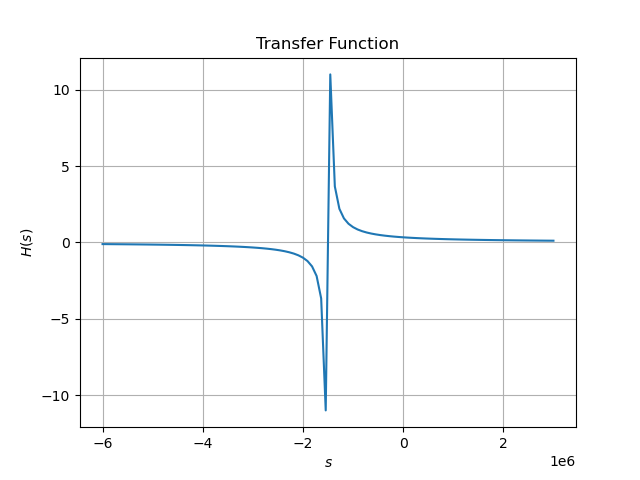
\includegraphics[width=\columnwidth]{./figs/4.3.png}
        \caption{Plot of $H(s)$}
        \label{fig-4.3}	
    \end{figure}
    
    Consider the frequency-domain transfer function by putting $s = \j\omega$
    \begin{align}
        H(\j\omega) &= \frac{5 \times 10^5}{\j\omega + 1.5 \times 10^6} \\
        \implies \abs{H(\j\omega)} &= \frac{5 \times 10^5}{\sqrt{\omega^2 + 2.25\times10^{12}}}
    \end{align}
    
    As $\omega$ increases, $\abs{H(\j\omega)}$ decreases
    
    In other words, the amplitude of high-frequency signals gets diminished and they get filtered out
    
    Therefore, this is a low-pass filter
    
    \item Using trapezoidal rule for integration, formulate the difference equation by considering 
    \begin{align}
        y(n) = y(t)\vert_{t=n}
    \end{align}
    
    \solution
    \begin{align}
        &\frac{v_c(t)}{R_1} + \frac{v_c(t) - v_2(t)}{R_2} + C_0\frac{\der{v_c}}{\der{t}} = 0 \\
        \implies &C_0\frac{\der{v_c}}{\der{t}} = \frac{2u(t)-v_c(t)}{R_2} - \frac{v_c(t)}{R_1} \\
        \implies &\left.v_c(t)\right|_{t=n}^{n+1} = \int_{n}^{n+1} \brak{\frac{2u(t)-v_c(t)}{R_2C_0} - \frac{v_c(t)}{R_1C_0}} \der{t}
    \end{align}
    
    By the trapezoidal rule of integration
    \begin{align}
        \int_a^b f(t) \der{t} \approx \frac{b-a}{2} (f(a) + f(b))
    \end{align}
    
    Consider $y(t) = v_c(t)$
    \begin{multline}
        y(n+1) - y(n) = \frac{1}{R_2C_0}\brak{u(n)+u(n+1)} \\
        - \frac12(y(n+1) + y(n))\brak{\frac{1}{R_1C_0} + \frac{1}{R_2C_0}}
    \end{multline}
    
    Thus, the difference equation is
    \begin{multline}
        y(n+1) \brak{1 + \frac{1}{2R_1C_0} + \frac{1}{2R_2C_0}} \\= y(n) \brak{1 - \frac{1}{2R_1C_0} - \frac{1}{2R_2C_0}} \\+ \frac{1}{R_2C_0}\brak{u(n)+u(n+1)}
    \end{multline}
    
    \item Find $H(z)$
    
    \solution Let $\z{y(n)} = Y(z)$
    
    On taking the $Z$-transform on both sides of the difference equation
    \begin{multline}
        zY(z)\brak{1 + \frac{1}{2R_1C_0} + \frac{1}{2R_2C_0}} \\= Y(z)\brak{1 - \frac{1}{2R_1C_0} - \frac{1}{2R_2C_0}} \\+ \frac{1}{R_2C_0} \brak{\frac{1}{1-z^{-1}} + \frac{z}{1-z^{-1}}}
    \end{multline}
    \begin{multline}
        Y(z)\brak{z + \frac{z}{2R_1C_0} + \frac{z}{2R_2C_0} - 1 + \frac{1}{2R_1C_0} + \frac{1}{2R_2C_0}} \\
        = \frac{1}{R_2C_0} \frac{1+z}{1-z^{-1}}
    \end{multline}
    
    Also
    \begin{align}
        v_2(t) &= 2 &&\forall t \ge 0\\
        \implies x(n) &= 2u(n) \\
        \implies X(z) &= \frac{2}{1-z^{-1}} &&\abs{z} > 1
    \end{align}
    
    Thus, the transfer function in $z$-domain is
    \begin{align}
        H(z) &= \frac{Y(z)}{X(z)} \\
        &= \frac{\frac{1+z}{2R_2C_0}}{z + \frac{z}{2R_1C_0} + \frac{z}{2R_2C_0} - 1 + \frac{1}{2R_1C_0} + \frac{1}{2R_2C_0}} \\
        &= \frac{\frac{1 + z^{-1}}{2R_2C_0}}{1 + \frac{1}{2R_1C_0} + \frac{1}{2R_2C_0} - z^{-1} + \frac{z^{-1}}{2R_1C_0} + \frac{z^{-1}}{2R_2C_0}}
    \end{align}
    
    On substituting the values
    \begin{align}
        H(z) &= \frac{2.5\times10^5 (1+z^{-1})}{7.5\times10^5 + 1 + (7.5\times10^5 - 1)z^{-1}}
    \end{align}
    
    with the ROC being
    \begin{align}
        \abs{z} &> \max\brak{1, \abs{\frac{7.5\times10^5 - 1}{7.5\times10^5 + 1}}} \\
        \implies \abs{z} &> 1
    \end{align}
    
    \item How can you obtain $H(z)$ from $H(s)$?
    
    \solution The $Z$-transform can be obtained from the Laplace transform by the substitution
    \begin{align}
        s &= \frac{2}{T} \frac{1-z^{-1}}{1+z^{-1}}
    \end{align}
    where $T$ is the step size of the trapezoidal rule ($1$ in our case)
    
    This is known as the bilinear transform
    
    Thus
    \begin{align}
        H(z) &= \frac{\frac{1}{R_2C_0}}{2\frac{1-z^{-1}}{1+z^{-1}} + \frac{1}{R_1C_0} + \frac{1}{R_2C_0}} \\
        &= \frac{\frac{1 + z^{-1}}{2R_2C_0}}{1-z^{-1}	 + \brak{\frac{1}{2R_1C_0} + \frac{1}{2R_2C_0}}(1 + z^{-1})} \\
        &= \frac{\frac{1 + z^{-1}}{2R_2C_0}}{1 + \frac{1}{2R_1C_0} + \frac{1}{2R_2C_0} - z^{-1} + \frac{z^{-1}}{2R_1C_0} + \frac{z^{-1}}{2R_2C_0}} \\
        &= \frac{2.5\times10^5 (1+z^{-1})}{7.5\times10^5 + 1 + (7.5\times10^5 - 1)z^{-1}}
    \end{align}
    which is the same as what we obtained earlier


\item Find $v(n)$. Verify using ngspice and the differential equation.\\
\solution We have,
\begin{align}
    V(z) &= H(z)V_i(z) \\
         &= \frac{TV_2\tau\brak{1+z^{-1}}}{C_0R_2\brak{1-z^{-1}}\brak{\brak{2\tau+T}-\brak{2\tau-T}z^{-1}}} \\
         &= \frac{V_2\tau\brak{z+1}}{2C_0R_2}\sum_{k=-\infty}^{\infty}\brak{1-p^k}u(k)z^{-k}
\end{align}
where $p := \frac{2\tau-T}{2\tau+T}$. Thus,
\begin{align}
    v(n) = \frac{V_2\tau}{C_0R_2}\sbrak{u(n)\brak{1-p^n}+u(n+1)\brak{1-p^{n+1}}}
\end{align}
where $p := \frac{2\tau-1}{2\tau+1}$. We take $T = 10^{-7}$ as the
sampling interval. 
these equalities.\\
Download the following Python code that plots Fig. \ref{fig:vc0}
            \begin{lstlisting}
wget https://github.com/jarpula-Bhanu/EE3900/blob/main/Cktsig/codes/4.7.cir
wget https://github.com/jarpula-Bhanu/EE3900/blob/main/Cktsig/codes/4.7.py
            \end{lstlisting}
            
    Run the codes by executing
    \begin{lstlisting}
        ngspice 4.7.cir
        python 4.7.py
    \end{lstlisting}
\begin{figure}[!ht]
    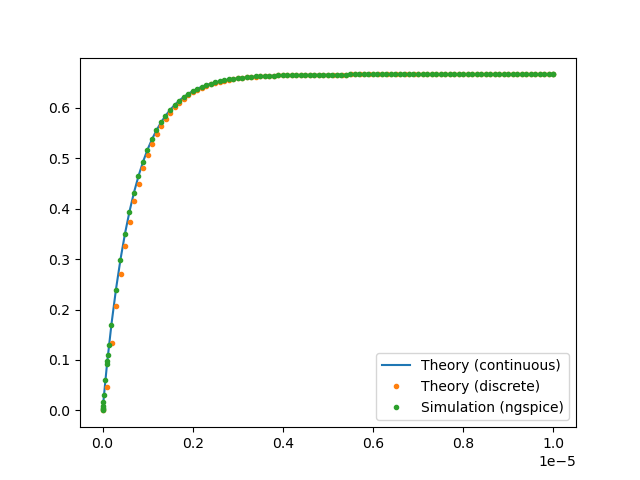
\includegraphics[width=\columnwidth]{figs/4.7.png}
    \caption{Representation of output across $C_0$.}
    \label{fig:vc0}
\end{figure}
            \end{enumerate}

\end{document}